\documentclass[14pt]{article}
\usepackage{../../report-tex/styles}


\begin{document}

    \titlewithlabnum{5}

    \tableofcontents
    \newpage


    \section{Мета:}
    Мета роботи – отримати вміння та навички програмувати багатовіконний інтерфейс програми на С++ в об’єктно-орієнтованому стилі.


    \section{Завдання:}
    1. Створити у середовищі MS Visual Studio C++ проект Desktop Application з ім’ям Lab5. \\
    2. Написати вихідний текст програми згідно варіанту завдання. \\
    3. Скомпілювати вихідний текст і отримати виконуваний файл програми. \\
    4. Перевірити роботу програми. Налагодити програму. \\
    5. Проаналізувати та прокоментувати результати та вихідний текст програми. \\
    6. Оформити звіт. \\

    \subsection{Варіант: }
    1. Для усіх варіантів завдань необхідно дотримуватися вимог та положень, викладених вище у порядку виконання роботи та методичних рекомендаціях. \\
    2. Номер варіанту завдання дорівнює номеру зі списку студентів у журналі. Студенти з парним номером (2, 4, 6, . . .) програмують об’єкт класу MyEditor на основі класичної реалізації Singleton. \\
    \begin{align}
        22 \bmod 2 = 0
    \end{align}
    3. Усі кольори та стилі геометричних форм – як у попередньої лаб. роботі №4. \\
    4. Запрограмувати вікно таблиці. Для його відкриття та закриття передбачити окремий пункт меню. Вікно таблиці повинно автоматично закриватися при виході з програми. \\
    5. Вікно таблиці – немодальне вікно діалогу. Таблиця повинна бути запрограмована як клас у окремому модулі. Інтерфейс модуля у вигляді оголошення класу таблиці \\
    6. Запрограмувати запис файлу множини об’єктів, що вводяться \\
    7. Оголошення класів для усіх типів об'єктів робити у окремих заголовочних файлах *.h, а визначення функцій членів – у окремих файлах *.cpp. Таким чином, програмний код для усіх наявних типів об'єктів розподілюється по множині окремих модулів. \\
    8. Ієрархія класів та побудова модулів повинні бути зручними для можливостей додавання нових типів об'єктів без переписування коду вже існуючих модулів. \\
    9. У звіті повинна бути схема успадкування класів – діаграма класів. Побудувати діаграму класів засобами Visual Studio C++. \\
    11. Бонуси-заохочення, які можуть суттєво підвищити оцінку лабораторної роботи. Оцінка підвищується за виконання кожного пункту, з наведених нижче: \\
    1). Якщо у вікні таблиці буде передбачено, щоб користувач міг виділити курсором рядок таблиці і відповідний об’єкт буде якось виділятися на зображенні у головному вікні. \\
    2). Якщо у вікні таблиці користувач може виділити курсором рядок таблиці і відповідний об’єкт буде вилучено з масиву об’єктів. 89 \\
    При виконанні бонусів 1 та 2 забороняється робити для цього нові залежності модуля my\_table від інших .cpp файлів. Тоді як надіслати повідомлення (наприклад, про виділення користувачем якогось рядка таблиці) від вікна таблиці клієнту цього вікна (наприклад, коду головного файлу .cpp)? Підказки можна знайти у матеріалі лекції стосовно технології Callback, а також патернів Observer, Listener. \\
    3). Якщо програма не тільки записує у файл опис множини об’єктів, а ще й здатна завантажити такий файл і відобразити відповідні об’єкти у головному вікні та вікні таблиці \\


    \section{Текст програми:}
    \subsection{Module: com.github.erotourtes.drawing.editor}
\lstinputlistingukr{DmProcessor.kt}{../src/main/kotlin/com/github/erotourtes/drawing/editor/DmProcessor.kt}
\lstinputlistingukr{Editor.kt}{../src/main/kotlin/com/github/erotourtes/drawing/editor/Editor.kt}
\lstinputlistingukr{Editors.kt}{../src/main/kotlin/com/github/erotourtes/drawing/editor/Editors.kt}
\lstinputlistingukr{ShapesList.kt}{../src/main/kotlin/com/github/erotourtes/drawing/editor/ShapesList.kt}

\subsection{Module: 1.0}
\lstinputlistingukr{MANIFEST.MF}{../src/main/resources/META-INF/MANIFEST.MF}

\subsection{Module: com.github.erotourtes.view}
\lstinputlistingukr{MainController.kt}{../src/main/kotlin/com/github/erotourtes/view/MainController.kt}
\lstinputlistingukr{MainView.kt}{../src/main/kotlin/com/github/erotourtes/view/MainView.kt}
\lstinputlistingukr{MenuBar.kt}{../src/main/kotlin/com/github/erotourtes/view/MenuBar.kt}
\lstinputlistingukr{ToolBar.kt}{../src/main/kotlin/com/github/erotourtes/view/ToolBar.kt}

\subsection{Module: com.github.erotourtes.app}
\lstinputlistingukr{MyApp.kt}{../src/main/kotlin/com/github/erotourtes/app/MyApp.kt}

\subsection{Module: com.github.erotourtes.drawing}
\lstinputlistingukr{CanvasPane.kt}{../src/main/kotlin/com/github/erotourtes/drawing/CanvasPane.kt}
\lstinputlistingukr{EditorHandler.kt}{../src/main/kotlin/com/github/erotourtes/drawing/EditorHandler.kt}

\subsection{Module: com.github.erotourtes.drawing.shape}
\lstinputlistingukr{Shape.kt}{../src/main/kotlin/com/github/erotourtes/drawing/shape/Shape.kt}
\lstinputlistingukr{Shapes.kt}{../src/main/kotlin/com/github/erotourtes/drawing/shape/Shapes.kt}

\subsection{Module: com.github.erotourtes.styles}
\lstinputlistingukr{ToolbarStyles.kt}{../src/main/kotlin/com/github/erotourtes/styles/ToolbarStyles.kt}

\subsection{Module: com.github.erotourtes.utils}
\lstinputlistingukr{Dimension.kt}{../src/main/kotlin/com/github/erotourtes/utils/Dimension.kt}
\lstinputlistingukr{ExtensionFunctions.kt}{../src/main/kotlin/com/github/erotourtes/utils/ExtensionFunctions.kt}
\lstinputlistingukr{Utils.kt}{../src/main/kotlin/com/github/erotourtes/utils/Utils.kt}




    \section{Ілюстрації:}
    \begin{figure}[H]
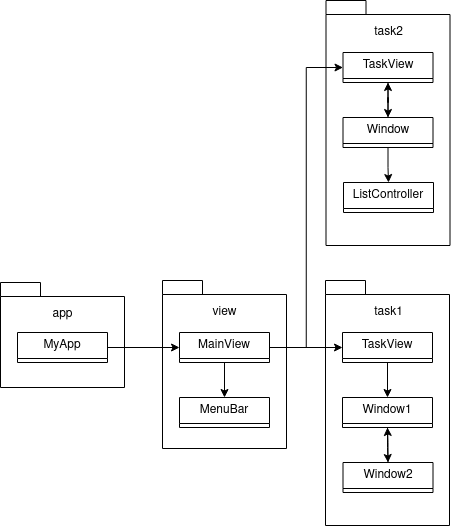
\includegraphics[width=10cm]{1}
\centering
\end{figure}



    \section{Висновки:}
    Отже, я отримав вміння та навички проектування багатовіконних програм на С++ в об’єктно-орієнтованому стилі.
\end{document}
